\documentclass[spanish,a4paper,14pt,oneside]{extreport}
\usepackage[utf8]{inputenc}
\usepackage[spanish]{babel}
%%%%%%%%%%%%%%%%%%%%%%%%%%%%%%%%%%%%%%%%%%%%%%%%%%%%%%%%%%%%%%%%%%%%%%%%%%%%%%%
% Next 3+3 lines select PDF or PS output respectively (comment as apropriate)
% To switch from PDF and PS comment/uncomment here
% and change correspondingly the Makefile
%
\usepackage[pdftex]{color}
\usepackage[pdftex]{graphicx}
\graphicspath{{FIGURES/}}
%\usepackage[dvips]{color}
%%\usepackage[dvips]{graphicx}
%\graphicspath{{FIGURES/}}
%%%%%%%%%%%%%%%%%%%%%%%%%%%%%%%%%%%%%%%%%%%%%%%%%%%%%%%%%%%%%%%%%%%%%%%%%%%%%%%
\usepackage{alltt}
\usepackage{algorithm}
\usepackage{algorithmic}
\usepackage{multirow}
\usepackage[top=2cm, bottom=2cm, left=2cm, right=2cm]{geometry}
%%%%%%%%%%%%%%%%%%%%%%%%%%%%%%%%%%%%%%%%%%%%%%%%%%%%%%%%%%%%%%%%%%%%%%%%%%%%%%%
\newcommand{\SONY}{{\sc Sony}}
\newcommand{\INTEL}{\textsf{\textsc{I}ntel}}

%%% Traducimos el pseudocodigo
\renewcommand{\algorithmicwhile}{\textbf{mientras}}
\renewcommand{\algorithmicend}{\textbf{fin}}
\renewcommand{\algorithmicdo}{\textbf{hacer}}
\renewcommand{\algorithmicif}{\textbf{si}}
\renewcommand{\algorithmicthen}{\textbf{entonces}}
\renewcommand{\algorithmicrepeat}{\textbf{repetir}}
\renewcommand{\algorithmicuntil}{\textbf{hasta que}}
\renewcommand{\algorithmicelse}{\textbf{en otro caso}}
\renewcommand{\algorithmicfor}{\textbf{para}}

%\newcommand{\RETURN}{\textbf{retornar} }
\newcommand{\RET}{\STATE \textbf{retornar} }
\newcommand{\TO}{\textbf{hasta} }
\newcommand{\AND}{\textbf{y} }
\newcommand{\OR}{\textbf{o} }

%%%%%%%%%%%%%%%%% Creamos un entorno para listar código fuente %%%%%%%%%%%%%%%
\newenvironment{sourcecode}
{\begin{list}{}{\setlength{\leftmargin}{1em}}\item\scriptsize\bfseries}
{\end{list}}

\newenvironment{littlesourcecode}
{\begin{list}{}{\setlength{\leftmargin}{1em}}\item\tiny\bfseries}
{\end{list}}

\newenvironment{summary}
{\par\noindent\begin{center}\textbf{Abstract}\end{center}\begin{itshape}\par\noindent}
{\end{itshape}}

\newenvironment{keywords}
{\begin{list}{}{\setlength{\leftmargin}{1em}}\item[\hskip\labelsep \bfseries Keywords:]}
{\end{list}}

\newenvironment{palabrasClave}
{\begin{list}{}{\setlength{\leftmargin}{1em}}\item[\hskip\labelsep \bfseries Palabras clave:]}
{\end{list}}

%%%%%%%%%%%%%%%%%%%%%%%%%%%%%%%%%%%%%%%%%%%%%%%%%%%%%%%%%%%%%%%%%%%%%%%%%%%%%%%
\begin{document}
\renewcommand\listtablename{Índice de Tablas}      % Estos comandos (al haber cargado babel)
\renewcommand\listfigurename{Índice de Figuras}    % Han de ir inmediatamente después del begin{document}

%%%%%%%%%%%%%%%%%%%%%%%%%%%%%%%%%%%%%%%%%%%%%%%%%%%%%%%%%%%%%%%%%%%%%%%%%%%%%%%
% First Page
%%%%%%%%%%%%%%%%%%%%%%%%%%%%%%%%%%%%%%%%%%%%%%%%%%%%%%%%%%%%%%%%%%%%%%%%%%%%%%%

\pagestyle{empty}
\thispagestyle{empty}


\newcommand{\HRule}{\rule{\linewidth}{1mm}}
\setlength{\parindent}{0mm}
\setlength{\parskip}{0mm}

\vspace*{\stretch{0.5}}

\centering{
\includegraphics[width=0.3\textwidth]{images/logo_vertical}
\vspace*{\stretch{0.5}}
\begin{center}
{\Huge Trabajo de Fin de Máster}
\end{center}

\HRule
\begin{flushright}
        {\Huge Título} \\[2.5mm]
        {\Large \textit{Title in English} .} \\[5mm]
        {\Large Autor} \\[5mm]


\end{flushright}
\HRule
\vspace*{\stretch{2}}
\begin{center}
  \Large La Laguna, \today
\end{center}

\setlength{\parindent}{5mm}

%%%%%%%%%%%%%%%%%%%%%%%%%%%%%%%%%%%%%%%%%%%%%%%%%%%%%%%%%%%%%%%%%%%%%%%%%%%%%%%
% Signature page (add the official stamp)
%%%%%%%%%%%%%%%%%%%%%%%%%%%%%%%%%%%%%%%%%%%%%%%%%%%%%%%%%%%%%%%%%%%%%%%%%%%%%%%
\newpage
%\cleardoublepage
\thispagestyle{empty}

D. {\bf Nombre Apellido1 Apellido2}, con DNI número 12.345.678-X
profesor
Titular de Universidad
adscrito al Departamento
de Nombre del Departamento
de la Universidad de La Laguna, como tutor

\bigskip
D. {\bf Nombre Apellido1 Apellido2}, con DNI número 12.345.678-X
profesor
Titular de Universidad
adscrito al Departamento
de Nombre del Departamento
de la Universidad de La Laguna, como cotutor

\bigskip
\bigskip
{\bf C E R T I F I C A (N)}

\bigskip
\bigskip
\bigskip
Que la presente memoria titulada:

\bigskip
``{\it Título del Trabajo.}''

\bigskip
\bigskip
\bigskip

\noindent ha sido realizada bajo su dirección por D. {\bf Nombre Apellido1 Apellido2},
con DNI número 12.345.678-X.

\bigskip
\bigskip

Y para que así conste, en cumplimiento de la legislación vigente y a los efectos
oportunos firman la presente en La Laguna a \today

%\cleardoublepage
\newpage
%%%%%%%%%%%%%%%%%%%%%%%%%%%%%%%%%%%%%%%%%%%%%%%%%%%%%%%%%%%%%%%%%%%%%%%%%%%%%%%
\thispagestyle{empty}

{ \flushright

\begin{LARGE}
Agradecimientos
\end{LARGE}

\hspace{3mm}

\begin{large}


\hspace{3mm}
XXX

\hspace{3mm}
XXX


\hspace{3mm}
XXX


\hspace{3mm}
XXX


\end{large}

}

%%%%%%%%%%%%%%%%%%%%%%%%%%%%%%%%%%%%%%%%%%%%%%%%%%%%%%%%%%%%%%%%%%%%%%%%%%%%%%%%%
\newpage

\begin{huge}
Licencia
\end{huge}

\bigskip
* Si NO quiere permitir que se compartan las adaptaciones de tu obra
y NO quieres permitir usos comerciales de tu obra indica:


\centering{
\includegraphics[width=0.2\textwidth]{images/by-nc-nd_88x31}
\begin{center}
{\Large \copyright~Esta obra está bajo una licencia de Creative Commons Reconocimiento-NoComercial-SinObraDerivada 4.0 Internacional.
}
\end{center}


\bigskip
* Si quiere permitir que se compartan las adaptaciones de tu obra mientras se comparta de la misma manera
y NO quieres permitir usos comerciales de tu obra indica:

\centering{
\includegraphics[width=0.2\textwidth]{images/by-nc-sa_88x31}
\begin{center}
{\Large \copyright~Esta obra está bajo una licencia de Creative Commons Reconocimiento-NoComercial-CompartirIgual 4.0 Internacional.
}
\end{center}



\bigskip
* Si quiere permitir que se compartan las adaptaciones de tu obra
y NO quieres permitir usos comerciales de tu obra indica:

\centering{
\includegraphics[scale=1.5]{images/by-nc_88x31}}
\begin{center}
{\Large \copyright~Esta obra está bajo una licencia de Creative Commons Reconocimiento-NoComercial 4.0 Internacional.
}
\end{center}

\newpage

\bigskip
*Si NO quiere permitir que se compartan las adaptaciones de tu obra
y quieres permitir usos comerciales de tu obra indica:

\centering{
\includegraphics[scale=1.5]{images/by-nd_88x31}}
\begin{center}
{\Large \copyright~Esta obra está bajo una licencia de Creative Commons Reconocimiento-SinObraDerivada 4.0 Internacional.
}
\end{center}


\bigskip
* Si quiere permitir que se compartan las adaptaciones de tu obra mientras se comparta de la misma manera
y quieres permitir usos comerciales de tu obra (licencia de Cultura Libre) indica:

\centering{
\includegraphics[scale=1.5]{images/by-sa_88x31}}
\begin{center}
{\Large \copyright~Esta obra está bajo una licencia de Creative Commons Reconocimiento-CompartirIgual 4.0 Internacional.
}
\end{center}


\bigskip
* Si quiere permitir que se compartan las adaptaciones de tu obra
y quieres permitir usos comerciales de tu obra (licencia de Cultura Libre) indica:

\centering{
\includegraphics[scale=1.5]{images/by_88x31}}
\begin{center}
{\Large \copyright~Esta obra está bajo una licencia de Creative Commons Reconocimiento 4.0 Internacional.
}
\end{center}



%%%%%%%%%%%%%%%%%%%%%%%%%%%%%%%%%%%%%%%%%%%%%%%%%%%%%%%%%%%%%%%%%%%%%%%%%%%%%%%
\newpage  %\cleardoublepage
\begin{abstract}
{\em

El objetivo de este trabajo ha sido ....
%
bla, bla, bla
%
bla, bla, bla
%
bla, bla, bla

\bigskip
Se ha incluido el apartado de 'Licencia' con todas las posibles licencias abiertas (Creative Commons).
En el caso en que se decida hacer público el contenido de la memoria, habrá que elegir una de ellas
(y borrar las demás).
La decisión de hacer pública o no la memoria se indica en el momento de subir la memoria a la Sede Electrónica de la ULL, paso necesario en el proceso de presentación del Trabajo Fin de Máster.

\bigskip
El documento de memoria debe tener un máximo de 100 páginas.

\bigskip
No se deben dejar páginas en blanco al comenzar un capítulo, ya que el documento no está pensado para ser
impreso sino leído con un lector de ficheros en formato PDF.

\bigskip
También es recomendable limitar el tamaño de los márgenes ya que, al firmar digitalmente en la sede
electrónica, se coloca un marco alrededor del texto original.

\bigskip
El tipo de letra base ha de ser de 14 puntos.
}

\begin{palabrasClave}
Palabra clave1, Palabra clave2, $\ldots$
\end{palabrasClave}

\end{abstract}
%%%%%%%%%%%%%%%%%%%%%%%%%%%%%%%%%%%%%%%%%%%%%%%%%%%%%%%%%%%%%%%%%%%%%%%%%%%%%%%

%%%%%%%%%%%%%%%%%%%%%%%%%%%%%%%%%%%%%%%%%%%%%%%%%%%%%%%%%%%%%%%%%%%%%%%%%%%%%%%
\newpage  %\cleardoublepage
\begin{summary}
{\em
Insert here an abstract in an EU language (preferably English)
}

\begin{keywords}
Keyword1, Keyword2, Keyword3, ...
\end{keywords}

\end{summary}
%%%%%%%%%%%%%%%%%%%%%%%%%%%%%%%%%%%%%%%%%%%%%%%%%%%%%%%%%%%%%%%%%%%%%%%%%%%%%%%

%%%%%%%%%%%%%%%%%%%%%%%%%%%%%%%%%%%%%%%%%%%%%%%%%%%%%%%%%%%%%%%%%%%%%%%%%%%%%%%
\newpage{\pagestyle{empty}}
\thispagestyle{empty}

%%%%%%%%%%%%%%%%%%%%%%%%%%%%%%%%%%%%%%%%%%%%%%%%%%%%%%%%%%%%%%%%%%%%%%%%%%%%%%%


\pagestyle{myheadings} %my head defined by markboth or markright
% No funciona bien \markboth sin "twoside" en \documentclass, pero al
% ponerlo se dan un montón de errores de underfull \vbox, con lo que no se
% ha puesto.
\markboth{Nombre del alumno}{Título del proyecto}

%%%%%%%%%%%%%%%%%%%%%%%%%%%%%%%%%%%%%%%%%%%%%%%%%%%%%%%%%%%%%%%%%%%%%%%%%%%%%%%
%Numeracion en romanos
\renewcommand{\thepage}{\roman{page}}
\setcounter{page}{1}

%%%%%%%%%%%%%%%%%%%%%%%%%%%%%%%%%%%%%%%%%%%%%%%%%%%%%%%%%%%%%%%%%%%%%%%%%%%%%%%

\tableofcontents

%%%%%%%%%%%%%%%%%%%%%%%%%%%%%%%%%%%%%%%%%%%%%%%%%%%%%%%%%%%%%%%%%%%%%%%%%%%%%%%
\newpage{\pagestyle{empty}}

\listoffigures

%%%%%%%%%%%%%%%%%%%%%%%%%%%%%%%%%%%%%%%%%%%%%%%%%%%%%%%%%%%%%%%%%%%%%%%%%%%%%%%
\newpage{\pagestyle{empty}}

\listoftables

%%%%%%%%%%%%%%%%%%%%%%%%%%%%%%%%%%%%%%%%%%%%%%%%%%%%%%%%%%%%%%%%%%%%%%%%%%%%%%%
\newpage{\pagestyle{empty}}

%%%%%%%%%%%%%%%%%%%%%%%%%%%%%%%%%%%%%%%%%%%%%%%%%%%%%%%%%%%%%%%%%%%%%%%%%%%%%%%
%Numeracion a partir del capitulo I
\renewcommand{\thepage}{\arabic{page}}
\setcounter{page}{1}


\chapter{Introducción}
\label{chapter:intro}

%%%%%%%%%%%%%%%%%%%%%%%%%%%%%%%%%%%%%%%%%%%%%%%%%%%%%%%%%%%%%%%%%%%%%%%%%%%%%
% Chapter 1: Introducción 
%%%%%%%%%%%%%%%%%%%%%%%%%%%%%%%%%%%%%%%%%%%%%%%%%%%%%%%%%%%%%%%%%%%%%%%%%%%%%%%

%---------------------------------------------------------------------------------
\section{Antecedentes}
\label{1:sec:1}

La World Wide Web está sujeta a un cambio continuo. La llegada de HTML5, la creciente importancia
de AJAX y de la programación en el lado del cliente, las nuevas fronteras de la Web Semántica, y la
explosión de las redes sociales son ejemplos de esta tendencia general.
\bigskip

Las aplicaciones web parecen evolucionar hacia entornos cada vez más ricos y flexibles en los que
los usuarios pueden acceder con facilidad a los documentos, publicar contenido, escuchar música, ver
vídeos, realizar dibujos e incluso jugar usando un navegador. Esta nueva clase de software ubicuo no
cesa de ganar momentum y promueve nuevas formas de interacción y cooperación.
\bigskip

Ante la rápida evolución del software, los sistemas de control de versiones han adquirido una mayor importancia dentro de la metodología del desarrollo del software: la gestión de las versiones del propio software se ha convertido en una actividad crítica. Estos sistemas han evolucionado a la par que el software, proporcionando nuevas funcionalidades y orientándose hacia la colaboración.

%---------------------------------------------------------------------------------
\section{Estado actual del arte}
\label{1:sec:2}

Actualmente, hay numerosos sistemas de control de versiones. Todos ellos proporcionan mecanismos de almacenamiento del código, de modificación y de consulta histórica del mismo, a la vez que proporcionan un entorno colaborativo en el que los usuarios pueden colaborar e interactuar entre sí.

En el caso particular de GitHub, además de proporcionar lo mencionado anteriormente, observando el creciente número de estudiantes que utiliza la plataforma, ha creado herramientas específicas para facilitar sus desarrollos (ej: Student Developer Pack) y provee a profesores de herramientas para gestionar dichos desarrollos (ej: GitHub Classrooms).

Sin embargo, estas herramientas de gestión de desarrollos requieren una administración interactiva por parte del profesor. No cuentan aún con funcionalidades de automatización de tareas.

%---------------------------------------------------------------------------------
\section{Objetivos y actividades a realizar}
\label{1:sec:3}

En este proyecto se persigue integrar los conocimientos adquiridos durante los estudios del Máster y,
en especial, del itinerario de Tecnologías de la Información para solucionar problemas actuales de aplicaciones y servicios Web.

Los objetivos propuestos para alcanzar en este Trabajo de Fin de Máster ha sido los siguientes:
\begin{itemize}
  \item Conocer, dominar y practicar con lenguajes y herramientas de desarrollo de aplicaciones Web
    en el servidor (Node.js, npm).
  %\item Conocer, dominar y practicar con diferentes lenguajes y librerías en el cliente.
  \item Conocer, practicar y dominar de herramientas de Desarrollo Dirigido por Pruebas en entornos
web y la Integración Contínua.
  %\item Conocer, practicar y dominar diferentes lenguajes de marcas y de estilo.
  %\item Conocer, practicar y dominar diferentes mecanismos de despliegue.
  \item Conocer, practicar y familiarizarse con diferentes mecanismos de seguridad, autentificación
y autorización.
  \item Conocer, practicar y dominar diferentes herramientas colaborativas y de control de versiones.
  \item Conocer, practicar y dominar Metodologías Ágiles de desarrollo de software.
\end{itemize}
\bigskip

Y las actividades a realizar en el mismo son las que se describen a continuación:
\begin{itemize}
  \item Revisión bibliográfica y estado del arte.
  \item Desarrollar una herramienta de línea de comandos escrita en Node.js que permita automatizar tareas relacionadas con repositorios de GitHub:
  \begin{itemize}
    \item Autenticación con GitHub.
    \item Listar organizaciones, asignaciones y repositorios de GitHub del usuario.
    \item Automatizar la descarga de repositorios.
    \item Automatizar la ejecución de scripts en los repositorios (TDD, creación de entorno, evaluación de código...).
    \item Recopilar la información obtenida de la automatización de tareas y presentarla al usuario (PDF, HTML...).
  \end{itemize}
  \item Redacción de la memoria.
  \item Preparación de la presentación oral.
\end{itemize}

%---------------------------------------------------------------------------------
\section{Tecnología usada}
\label{1:sec:3}
 
Para llevar a cabo el desarrollo de esta herramienta se planteó realizar el desarrollo en \ceis{Node.js}, creando una librería modular que se pudiese instalar mediante el gestor de paquetes de Node.js (NPM).

\begin{figure}[H]
\begin{center}

\includegraphics[width=0.3\textwidth]{images/nodejs-logo}
\end{center}
\end{figure}

Además, se ha hecho uso de otras tecnologías enumeradas a continuación:
\begin{itemize}
  \item NPM            
\includegraphics[width=0.15\textwidth]{images/npm}
  \item GitHub         
\includegraphics[width=0.1\textwidth]{images/github}
  \item GitBook        
\includegraphics[width=0.3\textwidth]{images/gitbook}
  \item Travis-CI      
\includegraphics[width=0.3\textwidth]{images/travis-ci-logo}
\end{itemize}


%%%%%%%%%%%%%%%%%%%%%%%%%%%%%%%%%%%%%%%%%%%%%%%%%%%%%%%%%%%%%%%%%%%%%%%%%%%%%%%

\chapter{Título del Capítulo Dos}
\label{chapter:dos}

%%%%%%%%%%%%%%%%%%%%%%%%%%%%%%%%%%%%%%%%%%%%%%%%%%%%%%%%%%%%%%%%%%%%%%%%%%%%%%%
% Chapter 2: Desarrollo
%%%%%%%%%%%%%%%%%%%%%%%%%%%%%%%%%%%%%%%%%%%%%%%%%%%%%%%%%%%%%%%%%%%%%%%%%%%%%%%

%++++++++++++++++++++++++++++++++++++++++++++++++++++++++++++++++++++++++++++++

En el capítulo anterior se ha descrito el estado del arte actual y se ha definido el Trabajo de Fin de Máster, especificado los objetivos, actividades a desarrollar y las tecnologías empleadas para su desarrollo. A continuación, se describirá la metodología de trabajo seguida.

%++++++++++++++++++++++++++++++++++++++++++++++++++++++++++++++++++++++++++++++

\section{Metodología usada}
\label{2:sec:1}

Se ha llevado a cabo una metodología de trabajo ágil, común en el campo de la Ingeniería Informática, con reuniones quincenales en las que se definían una serie de tareas u objetivos (iteración) y que se presentaban la siguiente quincena. 
De este modo, con la entrega de prototipos funcionales de la aplicación, se han ido testeando, corrigiendo y mejorando las 
funcionalidades, al mismo tiempo que detectando problemas no contemplados en las fases previas de diseño.

Esta metodología, además, ha propiciado la generación de ideas que se han traducido en nuevas características.


%---------------------------------------------------------------------------------
\subsection{GitHub}
\label{subsec:2.1.1}

Para llevar a cabo esta metodología, se ha usado GitHub como herramienta de Control de Versiones (CVS).
Todo el código implementado se alojaba en dicha herramienta, permitiendo así su cómoda modificación y actualización.

[ Imagen ]

%\begin{figure}[H]
%\begin{center}
%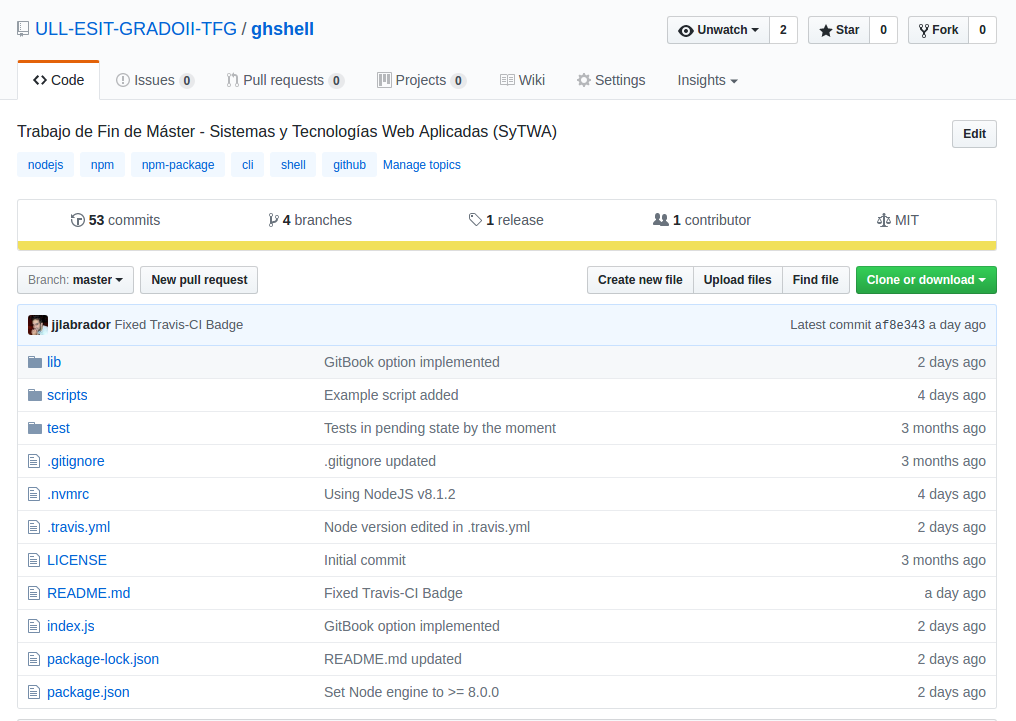
\includegraphics[width=\textwidth,height=0.58\textwidth]{images/github1.eps}
%\caption{Captura del repositorio de la gema en GitHub}
%\label{fig:github1}
%\end{center}
%\end{figure}

El trabajo se dividía en ramas, de modo que la versión estable de la aplicación (rama master) quedara aislada de la 
versión en desarrollo (rama develop) y de la rama experimental (rama test).


[ Imagen ]
%\begin{figure}[H]
%\begin{center}
%\includegraphics[width=0.47\textwidth]{images/github5.eps}
%\caption{Ramas del repositorio propio}
%\label{fig:github5}
%\end{center}
%\end{figure}


La documentación adicional para llevar a cabo los desarrollos de cada iteración, así como los problemas detectados, se anotaban en el apartado de issues con el fin de que quedara constancia de ello y se reflejara el estado en el que se encontraba cada uno.

\begin{figure}[H]
\begin{center}
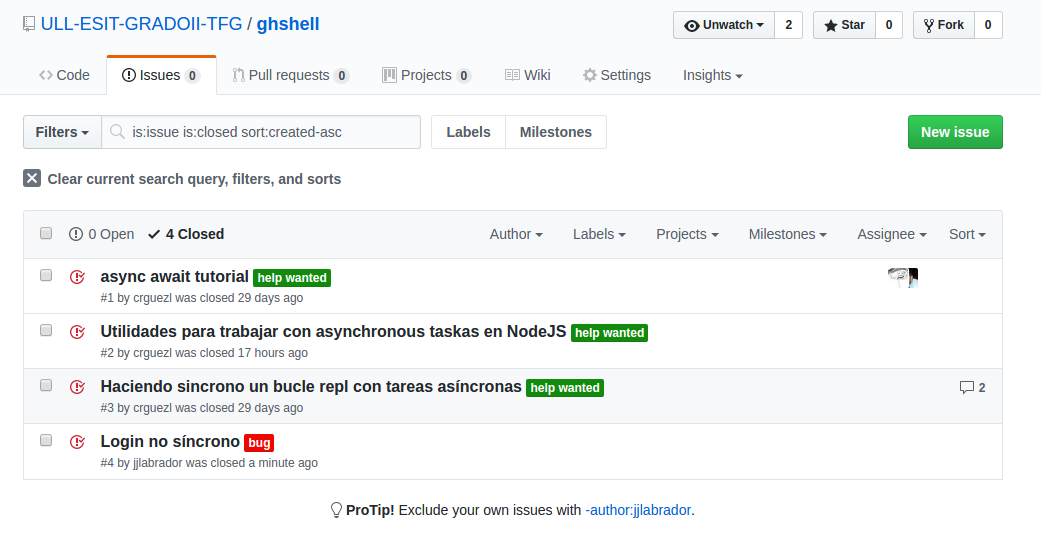
\includegraphics[width=1\textwidth]{images/github3}
\caption{Apartado de issues cerrados}
\label{fig:github3}
\end{center}
\end{figure}

%---------------------------------------------------------------------------------
\subsection{Travis-CI}
\label{subsec:2.1.2}

Como herramienta de integración continua, se ha utilizado Travis-CI, con el fin de asegurarnos el despliegue de la aplicación era satisfactorio tras cada cambio subido a la herramienta de control de versiones (GitHub).

\begin{figure}[H]
\begin{center}
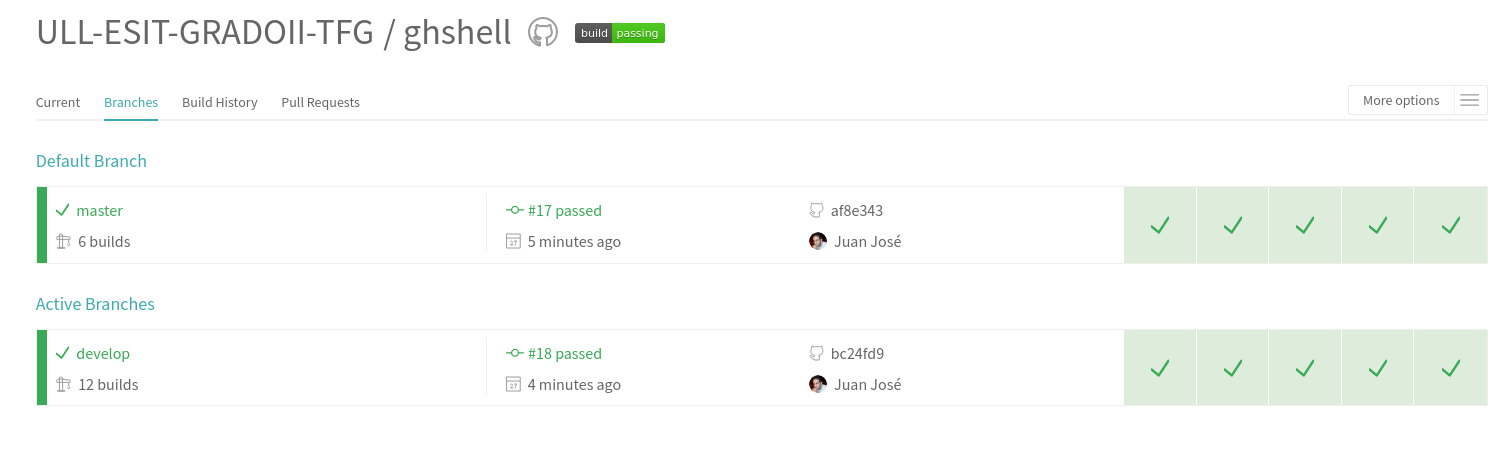
\includegraphics[width=1.1\textwidth]{images/travis-ci}
\caption{Herramienta de integración continua}
\label{fig:travisci}
\end{center}
\end{figure}

%---------------------------------------------------------------------------------
\subsection{Experiencia de usuario}
\label{subsec:2.1.3}

Por otra parte, el tutor del Trabajo de Fin de Máster ha hecho pruebas reales con el resultado de cada iteración. De este modo, se comprobaba el funcionamiento de la aplicación en un entorno real y se recibía un valioso feedback para coregir problemas o hacer mejoras en las siguientes iteraciones.


%%%%%%%%%%%%%%%%%%%%%%%%%%%%%%%%%%%%%%%%%%%%%%%%%%%%%%%%%%%%%%%%%%%%%%%%%%%%%%%
\newpage{\pagestyle{empty}}
\thispagestyle{empty}

\chapter{Título del Capítulo Tres}
\label{chapter:tres}

%%%%%%%%%%%%%%%%%%%%%%%%%%%%%%%%%%%%%%%%%%%%%%%%%%%%%%%%%%%%%%%%%%%%%%%%%%%%%%%
% Chapter 3: Resultados
%%%%%%%%%%%%%%%%%%%%%%%%%%%%%%%%%%%%%%%%%%%%%%%%%%%%%%%%%%%%%%%%%%%%%%%%%%%%%%%

%++++++++++++++++++++++++++++++++++++++++++++++++++++++++++++++++++++++++++++++

Finalizada la etapa de desarrollo del Trabajo de Fin de Máster, se procede a describir la herramienta implementada.


La herramienta se ha denominado \verb1ghshell1, abreviatura de 'GitHub Shell'. Se ha publicado en NPM\cite{URL:NPM} para su fácil distribución e instalación:

\begin{figure}[H]
\begin{center}
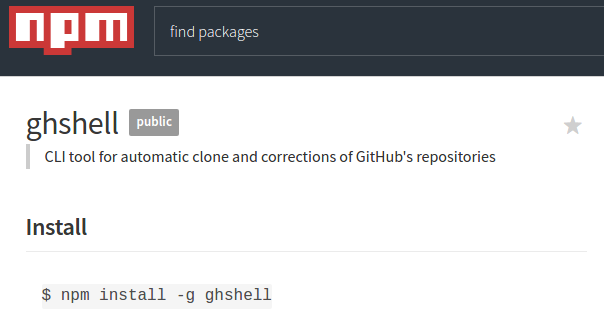
\includegraphics[width=0.8\textwidth]{images/npm1}
\caption{Página del gestor de paquetes NPM}
\label{fig:npm}
\end{center}
\end{figure}

Las funcionalidades implementadas en \verb|ghshell|, se describen a continuación.

%---------------------------------------------------------------------------------
\section{Funcionalidades requeridas}
\label{3:sec:1}

%------------------------------------------------------------------------------------------------------------
\subsection{Autenticación con GitHub}
\label{subsec:3.1.1}
    
    Una vez que el usuario se autentifica con GitHub, se genera un token personal, que se usa posteriormente para acceder a la API de Github. Este token se almacena cifrado en el equipo del usuario, por lo que las siguientes ocasiones que utilice la herramienta no hará falta que vuelva a iniciar sesión:
        
        \begin{figure}[H]
		\begin{center}
		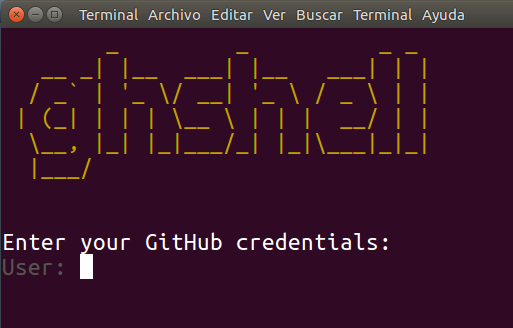
\includegraphics[width=0.7\textwidth]{images/ghshell1}
		\caption{Login de usuario}
		\label{fig:ghshell1}
		\end{center}
		\end{figure}
		
		\begin{figure}[H]
		\begin{center}
		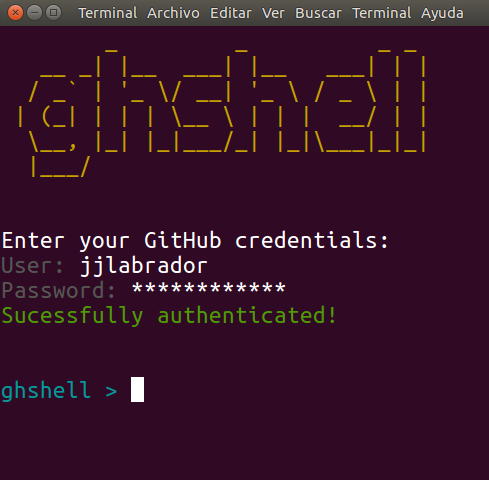
\includegraphics[width=0.6\textwidth]{images/ghshell2-1}
		\caption{Usuario autenticado}
		\label{fig:ghshell2-1}
		\end{center}
		\end{figure}
		
		\begin{figure}[H]
		\begin{center}
		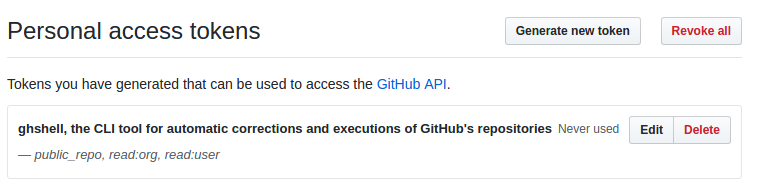
\includegraphics[width=1\textwidth]{images/ghshell2-3}
		\caption{Token personal en GitHub}
		\label{fig:ghshell2-3}
		\end{center}
		\end{figure}
		
		\begin{figure}[H]
		\begin{center}
		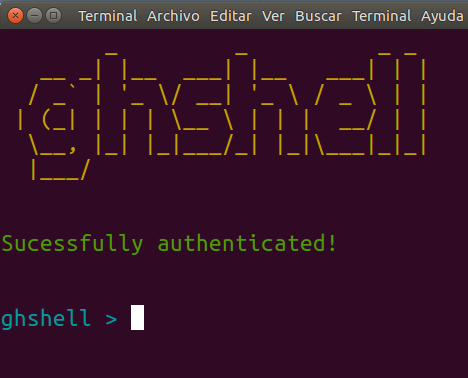
\includegraphics[width=0.6\textwidth]{images/ghshell2-4}
		\caption{Login automático una vez generado el token}
		\label{fig:ghshell2-4}
		\end{center}
		\end{figure}
		
	Si el usuario cierra sesión en la herramienta, se eliminará el token en GitHub y en el equipo:
	
		\begin{figure}[H]
		\begin{center}
		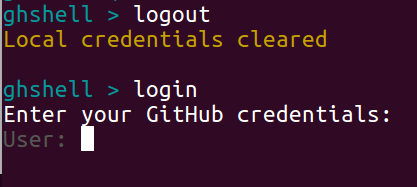
\includegraphics[width=0.6\textwidth]{images/ghshell2-2}
		\caption{Logout de usuario}
		\label{fig:ghshell2-2}
		\end{center}
		\end{figure}

%------------------------------------------------------------------------------------------------------------
\subsection{Listar organizaciones, asignaciones y repositorios de GitHub del usuario}
\label{subsec:3.1.2}   
    
    Con el comando \verb'orgs -l', se puede listar las organizaciones del usuario y usando \verb'repos -l', se listarán los repositorios del usuario. También se puede acceder 'virtualmente' a las organizaciones y listar los repositorios que contiene, así como las asignaciones.
\bigskip

    NOTA: se puede consultar toda la información referente a los comandos del programa en el Apéndice 2.
        
        \begin{figure}[H]
		\begin{center}
		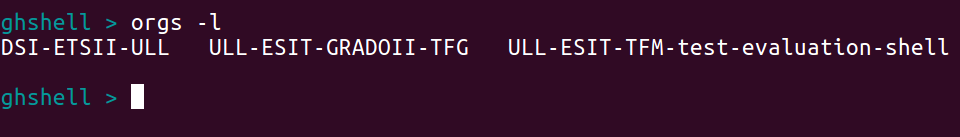
\includegraphics[width=0.9\textwidth]{images/ghshell3}
		\caption{Lista de organizaciones del usuario}
		\label{fig:ghshell3}
		\end{center}
		\end{figure}
		
		\begin{figure}[H]
		\begin{center}
		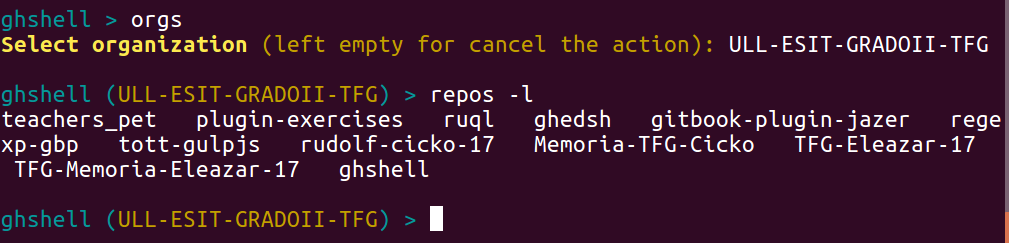
\includegraphics[width=0.9\textwidth]{images/ghshell4}
		\caption{Lista de repositorios de una organización}
		\label{fig:ghshell4}
		\end{center}
		\end{figure}
		
		\begin{figure}[H]
		\begin{center}
		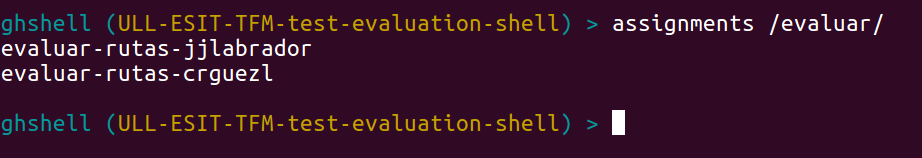
\includegraphics[width=0.9\textwidth]{images/ghshell5}
		\caption{Asignaciones dentro de otra organización}
		\label{fig:ghshell5}
		\end{center}
		\end{figure}
    Las asignaciones son un conjunto de repositorios que corresponden a una tarea asignada por los profesores a los alumnos.
		
	También es posible acceder 'virtualmente' a los repositorios y realizar acciones sobre ellos:
	
		\begin{figure}[H]
		\begin{center}
		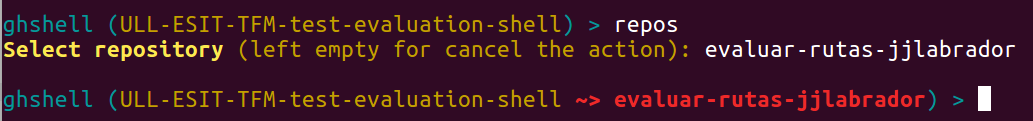
\includegraphics[width=1\textwidth]{images/ghshell5-1}
		\caption{Acceso a un repositorio de una organización}
		\label{fig:ghshell5-1}
		\end{center}
		\end{figure}

%------------------------------------------------------------------------------------------------------------
\subsection{Automatizar la descarga de repositorios}
\label{subsec:3.1.3}  
        	
    En función del contexto dónde nos encontremos dentro de la herramienta, podremos:
    \begin{itemize}
    	\item Clonar el repositorio en el que nos encontremos.
    	\item Clonar un repositorio determinado.
	    \item Clonar todos los repositorios que coincidan con una determinada expresión regular.
	    \item Clonar todos los repositorios de una asignación que coincidan con una determinada expresión
    \end{itemize}
    
    El clonado se realiza de manera asíncrona, por lo que podemos seguir trabajando mientras se clona(n) el/los repositorio(s). Se puede observar el estado de la clonación revisando el fichero de log que se genera cuyo nombre sigue el formato: \verb|nombre-repositorio -clone.log|.
    
    	\begin{figure}[H]
		\begin{center}
		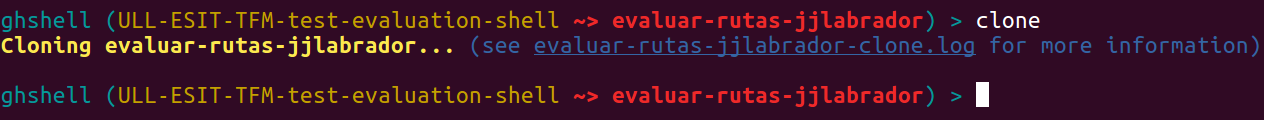
\includegraphics[width=1\textwidth]{images/ghshell6-3}
		\caption{Clonado del repositorio donde nos encontramos}
		\label{fig:ghshell6-3}
		\end{center}
		\end{figure}	

    Si clonamos repositorios que pertenecen a una organización, se creará una carpeta con el nombre de la organización y en su interior se guardarán los repositorios clonados.
    		
	Además, si clonamos repositorios que pertenecen a una asignación, también se creará una carpeta con el nombre de la asignación que los contendrá.
	
        \begin{figure}[H]
		\begin{center}
		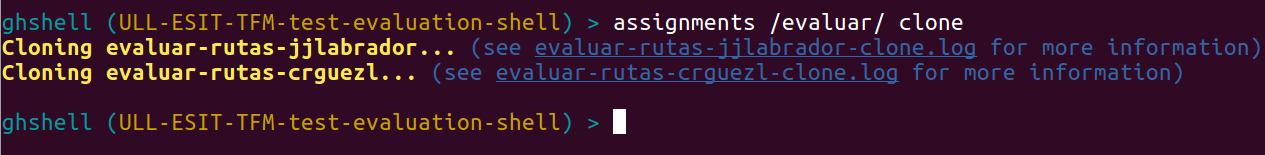
\includegraphics[width=1\textwidth]{images/ghshell6-1}
		\caption{Clonado de asignaciones que coinciden con una expresión regular}
		\label{fig:ghshell6-1}
		\end{center}
		\end{figure}	
		
		\begin{figure}[H]
		\begin{center}
		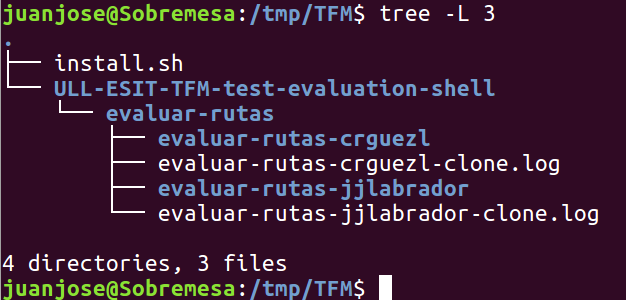
\includegraphics[width=0.7\textwidth]{images/ghshell6-2}
		\caption{Resultado del clonado}
		\label{fig:ghshell6-2}
		\end{center}
		\end{figure}
	
%------------------------------------------------------------------------------------------------------------
\subsection{Automatizar la ejecución de scripts en los repositorios}
\label{subsec:3.1.3} 
	    
    En función del contexto donde nos encontremos dentro de la herramienta, podremos:
    \begin{itemize}
    	\item Ejecutar un script en el repositorio en el que nos encontremos.
    	\item Ejecutar un script en un determinado repositorio.
	    \item Ejecutar un script en todos los repositorios que coincidan con una determinada expresión regular.
	    \item Ejecutar un script en todos los repositorios de una asignación coincidan con una determinada expresión regular.
    \end{itemize}
    
	La ruta del fichero del script puede ser absoluta o relativa. Estos scripts puede ser de cualquier tipo: TDD, creación de entorno, evaluación de código...
\bigskip

	La ejecución de cada script se ejecuta en un proceso hijo independiente pero, a diferencia del clonado, el script se ejecuta línea a línea de manera síncrona. Se puede observar el estado de la ejecución del script y los resultados revisando el fichero de log que se genera: \textless nombre-repositorio \textgreater - \textless nombre-script \textgreater .log
    	
    	\begin{figure}[H]
		\begin{center}
		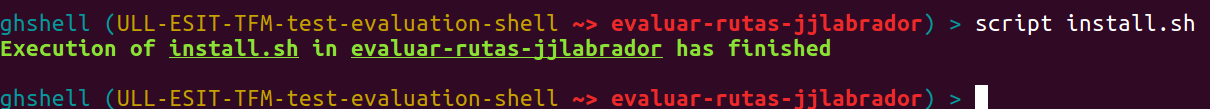
\includegraphics[width=1\textwidth]{images/ghshell7-3}
		\caption{Ejecución del script 'install.sh' en el repositorio actual}
		\label{fig:ghshell7-3}
		\end{center}
		\end{figure}
		
        \begin{figure}[H]
		\begin{center}
		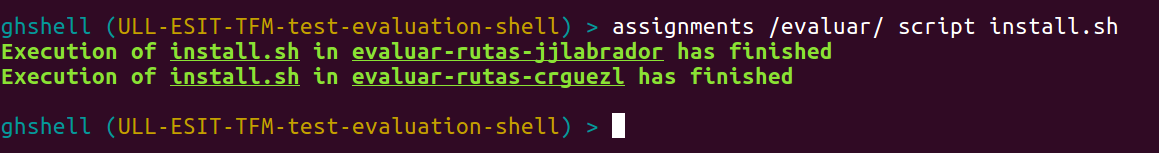
\includegraphics[width=1\textwidth]{images/ghshell7-1}
		\caption{Ejecución del script 'install.sh' en asignaciones que coinciden con una expresión regular}
		\label{fig:ghshell7-1}
		\end{center}
		\end{figure}	
		
		\begin{figure}[H]
		\begin{center}
		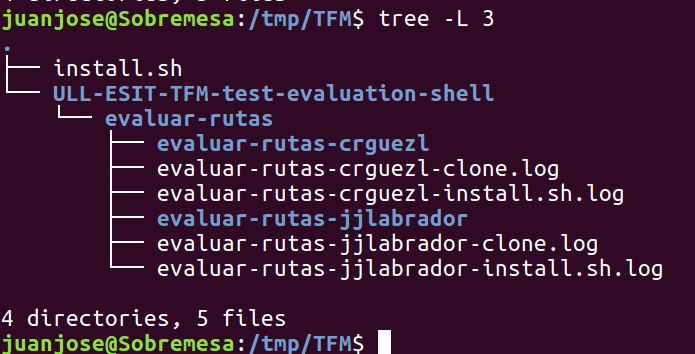
\includegraphics[width=0.7\textwidth]{images/ghshell7-2}
		\caption{Resultado de la ejecución del script 'install.sh'}
		\label{fig:ghshell7-2}
		\end{center}
		\end{figure}
		
%------------------------------------------------------------------------------------------------------------
\subsection{Recopilar la información obtenida de la automatización de tareas}
\label{subsec:3.1.4}

    Una vez ejecutados los scripts necesarios para evaluar un determinado repositorio, es posible generar un GitBook con el resultado de la ejecución de los mismos. Este libro se genera en formato PDF y en HTML.
\bigskip
    
    En función del contexto dónde nos encontremos dentro de la herramienta, podremos:
    \begin{itemize}
    	\item Crear un GitBook en el repositorio en el que nos encontremos.
    	\item Crear un GitBook en un determinado repositorio.
	    \item Crear un GitBook en todos los repositorios que coincidan con una determinada expresión regular.
	    \item Crear un GitBook en todos los repositorios de una asignación coincidan con una determinada expresión regular.
    \end{itemize}
        
        \begin{figure}[H]
		\begin{center}
		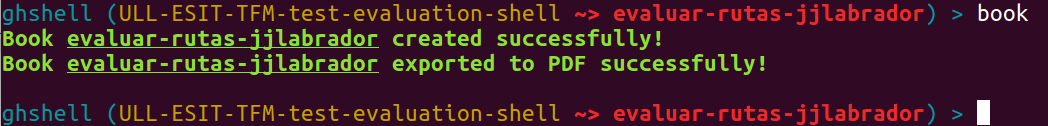
\includegraphics[width=1\textwidth]{images/ghshell8-3}
		\caption{Creación del Gitbook en el repositorio actual}
		\label{fig:ghshell8-3}
		\end{center}
		\end{figure}
		
        \begin{figure}[H]
		\begin{center}
		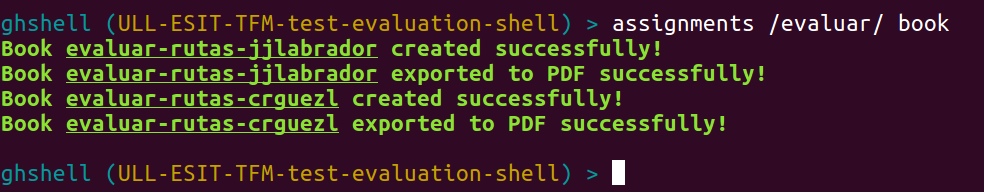
\includegraphics[width=1\textwidth]{images/ghshell8-1}
		\caption{Creación del Gitbook en asignaciones que coinciden con una expresión regular}
		\label{fig:ghshell8-1}
		\end{center}
		\end{figure}	
		
		\begin{figure}[H]
		\begin{center}
		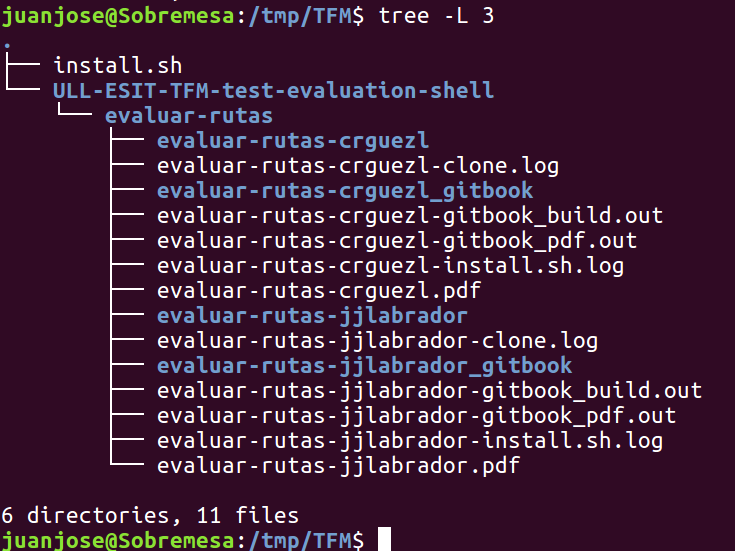
\includegraphics[width=0.7\textwidth]{images/ghshell8-2}
		\caption{Resultado de la creación del Gitbook}
		\label{fig:ghshell8-2}
		\end{center}
		\end{figure}
		
\newpage
%---------------------------------------------------------------------------------
\section{Funcionalidades extra}
\label{3:sec:2}

Además de las funcionales solicitadas en este Trabajo de Fin de Máster, se han añadido una serie de funcionalidades extra que, a pesar de no ser requeridas, brindan al usuario de una mejor experiencia de uso del programa:

\begin{itemize}
  \item Autocompletado de los comandos disponibles en función del contexto donde nos encontremos (nivel principal, organización o repositorio).
	\item Opción de ayuda que muestra la descripción de los comandos y cómo se utilizan. Esta ayuda varía dependiendo del contexto donde nos encontremos.
	\item Opción de visualizar el directorio de trabajo donde se ha ejecutado el programa. Útil para determinar rutas relativas de los scripts que se desean ejecutar.
	\item Opción para conocer el propietario de cada repositorio. En el caso de que el repositorio pertenezca a una organización, mostrará los contribuyentes de ese repositorio.
\end{itemize}

NOTA: se puede consultar toda la información referente a los comandos del programa en el Apéndice 2.

%---------------------------------------------------------------------------------
\section{Problemas encontrados y soluciones}
\label{3:sec:3}

A continuación se detallan los problemas encontrados durante la implementación de la herramienta y las soluciones encontradas para los mismos:

%---------------------------------------------------------------------------------
\subsection{Asincronía}
\label{subsec:3.3.1}

Una de las características más importantes del lenguaje JavaScript es la asincronía. Usa un modelo de operaciones de entrada/salida sin bloqueo y orientado a eventos, que lo hace ligero y eficiente. Sin embargo, algunas acciones que debía realizar esta herramienta debían de ser síncronas. Ejemplos son el login del usuario y ejecución de scripts.
\bigskip

{\normalsize {\bfseries Solución}}
\bigskip

La solución a este comportamiento pasó por realizar un amplio estudio de la documentación para usar mecanismos que permitieran bloquear la ejecución de la herramienta en las partes que deseábamos. Los mecanismos usados han sido:

\begin{itemize}
	\item Funciones síncronas del propio lenguaje.
	\item Promesas
	\item Métodos async/await
	\item Librerías con métodos implementados de manera síncrona.
\end{itemize}

%---------------------------------------------------------------------------------
\subsection{Autocompletado de comandos}
\label{subsec:3.3.2}

Para el manejo de los flujos de lectura y escritura de la herramienta, se ha utilizado la interfaz nativa de Node.js (Readline). Esta interfaz provee de una función de autocompletado para el texto que escribe el usuario.

Sin embargo, sólo funciona con la primera palabra (comando) que escribe. Tras investigar al respecto y buscar posibles librerías alternativas, no existía ninguna solución que corrigiera este comportamiento.
\bigskip

{\normalsize {\bfseries Solución}}
\bigskip

Realizando numerosas pruebas, se halló una manera propia de conseguir completar más de un comando en la misma línea. Cuando realice los test de aceptación pertinentes requeridos por la comunidad de Node, solicitaré un Pull Request a su repositorio con esta mejora.


%---------------------------------------------------------------------------------
\section{Perfil del usuario de ghshell}
\label{3:sec:4}

El uso de \verb|ghshell| está especialmente dirigido a un determinado grupo de profesores: nos referimos al perfil de un profesor, principalmente docente en alguna rama de Ingeniería, con conocimientos avanzados en programación y en herramientas de control de versiones.

No obstante, ya que la curva de aprendizaje de \verb|ghshell| no es excesiva y dado que el uso de las herramientas de control de versiones no se limita exclusivamente a repositorios de código fuente, se puede extender su uso para el resto de profesorado y usuarios con otros roles. Basta con tener claras unas nociones básicas de informática, junto con la lectura y asimilación previa de la documentación de la herramienta.


%%%%%%%%%%%%%%%%%%%%%%%%%%%%%%%%%%%%%%%%%%%%%%%%%%%%%%%%%%%%%%%%%%%%%%%%%%%%%%%

\chapter{Título del Capítulo Cuatro}
\label{chapter:cuatro}

%%%%%%%%%%%%%%%%%%%%%%%%%%%%%%%%%%%%%%%%%%%%%%%%%%%%%%%%%%%%%%%%%%%%%%%%%%%%%%%
% Chapter 4 : Título del Capítulo cuatro
%%%%%%%%%%%%%%%%%%%%%%%%%%%%%%%%%%%%%%%%%%%%%%%%%%%%%%%%%%%%%%%%%%%%%%%%%%%%%%%


Los capítulos intermedios servirán para cubrir los siguientes aspectos:
antecedentes, problemática o estado del arte, objetivos, fases y desarrollo del proyecto.


%++++++++++++++++++++++++++++++++++++++++++++++++++++++++++++++++++++++++++++++

En el capítulo ~\ref{chapter:intro} se describió bla, bla, bla.....




%%%%%%%%%%%%%%%%%%%%%%%%%%%%%%%%%%%%%%%%%%%%%%%%%%%%%%%%%%%%%%%%%%%%%%%%%%%%%%%
\newpage{\pagestyle{empty}}
\thispagestyle{empty}

\chapter{Conclusiones y líneas futuras}
\label{chapter:Conclusiones}

%%%%%%%%%%%%%%%%%%%%%%%%%%%%%%%%%%%%%%%%%%%%%%%%%%%%%%%%%%%%%%%%%%%%%%%%%%%%%
% Chapter 5: Summary and Conlusions
%%%%%%%%%%%%%%%%%%%%%%%%%%%%%%%%%%%%%%%%%%%%%%%%%%%%%%%%%%%%%%%%%%%%%%%%%%%%%%%

%++++++++++++++++++++++++++++++++++++++++++++++++++++++++++++++++++++++++++++++

This chapter is compulsory.
The memory should include an extended summary and conclusions in english. 

%---------------------------------------------------------------------------------
\section{First Section}
\label{5:sec:1}



%%%%%%%%%%%%%%%%%%%%%%%%%%%%%%%%%%%%%%%%%%%%%%%%%%%%%%%%%%%%%%%%%%%%%%%%%%%%%%%
\newpage{\pagestyle{empty}}
\thispagestyle{empty}

\chapter{Summary and Conclusions }
\label{chapter:ingles}

%%%%%%%%%%%%%%%%%%%%%%%%%%%%%%%%%%%%%%%%%%%%%%%%%%%%%%%%%%%%%%%%%%%%%%%%%%%%%
% Chapter 6: Presupuesto
%%%%%%%%%%%%%%%%%%%%%%%%%%%%%%%%%%%%%%%%%%%%%%%%%%%%%%%%%%%%%%%%%%%%%%%%%%%%%%%

%++++++++++++++++++++++++++++++++++++++++++++++++++++++++++++++++++++++++++++++

En este capítulo se especifica un presupuesto que indica cuánto costaría realizar este Trabajo de Fin de Máster
si se tratase de un trabajo encargado por un cliente.

%---------------------------------------------------------------------------------
\section{Introducción y coste por hora}
\label{6:sec:1}

Se definirá una tabla con la lista de actividades realizadas en este Trabajo de Fin de Máster. Otra columna indicará la duración en horas que se han empleado para dicha actividad junto con el precio por hora calculado.
\bigskip

El precio por hora que se considerará en este presupuesto es de 30\euro{}/hora.
\newpage
    
%---------------------------------------------------------------------------------
\section{Funcionalidades requeridas}
\label{6:sec:2}

%--------------------------------------------------------------------------
\begin{table}[!ht]
\begin{center}
\begin{tabular}{|p{80mm}|p{25mm}|p{20mm}|} \hline 
\textbf{Actividad} & \textbf{Duración} & \textbf{Precio} \\ \hline

Autenticación con GitHub &
xx horas &
xx \euro{}
\\
\hline

Listar organizaciones, asignaciones y repositorios &
xx horas &
xx \euro{}
\\
\hline

Automatizar la descarga de repositorios &
xx horas &
xx \euro{}
\\
\hline

Automatizar la ejecución de scripts en los repositorios &
xx horas &
xx \euro{}
\\
\hline

Exportar la información obtenida de la automatización de tareas &
xx horas &
xx \euro{}
\\
\hline \hline

{\bfseries Subtotal} &
{\bfseries xx horas} &
{\bfseries xx \euro{}}
\\
\hline

\end{tabular}
\end{center}
\caption{Tabla de actividades, duración y precios de las funcionalidades requeridas}
\label{table:resOthers1}
\end{table}



%---------------------------------------------------------------------------------
\section{Funcionalidades extra}
\label{6:sec:3}

%--------------------------------------------------------------------------
\begin{table}[!ht]
\begin{center}
\begin{tabular}{|p{80mm}|p{25mm}|p{20mm}|} \hline 
\textbf{Actividad} & \textbf{Duración} & \textbf{Precio} \\ \hline

Autocompletado de comandos según contexto &
xx horas &
xx \euro{}
\\
\hline

Opción de ayuda según contexto &
xx horas &
xx \euro{}
\\
\hline

Visualización del directorio de trabajo actual &
xx horas &
xx \euro{}
\\
\hline

Opción para conocer propietarios del repositorio &
xx horas &
xx \euro{}
\\
\hline \hline

{\bfseries Subtotal} &
{\bfseries xx horas} &
{\bfseries xx \euro{}}
\\
\hline

\end{tabular}
\end{center}
\caption{Tabla de actividades, duración y precios de las funcionalidades extra}
\label{table:resOthers2}
\end{table}


\newpage
%---------------------------------------------------------------------------------
\section{Coste y duración total}
\label{6:sec:4}

%--------------------------------------------------------------------------
\begin{table}[!ht]
\begin{center}
\begin{tabular}{|p{80mm}|p{25mm}|p{20mm}|} \hline 
\textbf{Actividad} & \textbf{Duración} & \textbf{Precio} \\ \hline

Funcionalidades requeridas &
xx horas &
xx \euro{}
\\
\hline

Funcionalidades extra &
xx horas &
xx \euro{}
\\
\hline \hline

{\bfseries Total} &
{\bfseries xx horas} &
{\bfseries xx \euro{}}
\\
\hline

\end{tabular}
\end{center}
\caption{Precio y duración total}
\label{table:resOthers3}
\end{table}




%%%%%%%%%%%%%%%%%%%%%%%%%%%%%%%%%%%%%%%%%%%%%%%%%%%%%%%%%%%%%%%%%%%%%%%%%%%%%%%
\newpage{\pagestyle{empty}}
\thispagestyle{empty}
\begin{appendix}

\chapter{Título del Apéndice 1}
\label{appendix:1}
\section{Algoritmo XXX}
\label{Apendice1:XXX}

\begin{center}
\begin{footnotesize}
\begin{verbatim}

***********************************************************************************
*
* Fichero .h
*
***********************************************************************************
*
* AUTORES
*   
*
* FECHA
*   
*
* DESCRIPCION
*   
*
************************************************************************************/

\end{verbatim}
\end{footnotesize}
\end{center}

\section{Algoritmo YYY}
\label{Apendice1:YYY}

\begin{center}
\begin{footnotesize}
\begin{verbatim}


/***********************************************************************************
 *
 * Fichero .h
 *
 ***********************************************************************************
 *
 * AUTORES
 *
 * FECHA
 *
 * DESCRIPCION
 *
 *
 ************************************************************************************/

\end{verbatim}
\end{footnotesize}
\end{center}


\chapter{Título del Apéndice 2}
\label{appendix:2}
El objetivo de esta gu\'{\i}a de usuario es proporcionar a los usuarios un ejemplo para la puesta a punto y ejecuci\'on de las 
funcionalidades implementadas en el gema RuQL durante el Trabajo de Fin de Grado.

%---------------------------------------------------------------------------------
\section{Instalación}
\label{Apendice2:instalacion}

Para instalar la gema, basta con ejecutar el siguiente comando:
\begin{verbatim}
[~]$ gem install ruql
\end{verbatim}


%---------------------------------------------------------------------------------
%---------------------------------------------------------------------------------

\section{Ejecución}
\label{Apendice2:ejecucion}

\begin{lstlisting}[language=JavaScript]
var foo = function(){
console.log('foo');
}
foo();
\end{lstlisting}
\bigskip

%---------------------------------------------------------------------------------
\subsection{Otras consideraciones}
\label{subsec:Apendice2.1}

Para que

\end{appendix}

%%%%%%%%%%%%%%%%%%%%%%%%%%%%%%%%%%%%%%%%%%%%%%%%%%%%%%%%%%%%%%%%%%%%%%%%%%%%%%%
\addcontentsline{toc}{chapter}{Bibliografía}
\bibliographystyle{plain}

\bibliography{memtfg}
\nocite{*}

%%%%%%%%%%%%%%%%%%%%%%%%%%%%%%%%%%%%%%%%%%%%%%%%%%%%%%%%%%%%%%%%%%%%%%%%%%%%%%%

\end{document}
